\section{Modules}
\SectionPage

\begin{frame}
  \frametitle{UI module}
  \begin{figure}[H]
    \centering
    \begin{tikzpicture}
  \node (window) [rectangle, draw, minimum height=7cm, minimum width=10cm] at (0, 0) {};
  \node (menu) [rectangle, draw, minimum height=0.5cm, minimum width=10cm] at (0, 3.25) {Menu};
  \node (tabs) [rectangle, draw, minimum height=0.25cm, minimum width=8cm] at (1, 2.75) {Tabs};
  \node (tab) [rectangle, draw, minimum height=0.25cm, minimum width=1cm] at (-2.5, 2.75) {Tab};
  \node (sidebar) [rectangle, draw, minimum height=6.5cm, minimum width=2cm] at (-4, -0.25) {Sidebar};
  \node (content) [rectangle, draw, minimum height=6.5cm, minimum width=8cm] at (1, -0.25) {Content};
\end{tikzpicture}
  \end{figure}
\end{frame}

\begin{frame}
  \frametitle{Menu}
  \begin{figure}
    \centering
    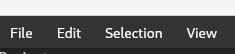
\includegraphics[width=0.5\textwidth]{./pics/menu-bar.png}
    \caption{
      Menu bar
    }
  \end{figure}
\end{frame}

\begin{frame}
  \frametitle{Dropdown menu}
  \begin{figure}
    \centering
    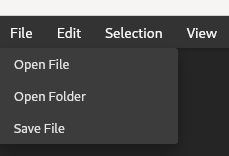
\includegraphics[width=0.5\textwidth]{./pics/menu-dropdown.png}
    \caption{
      Dropdown menu
    }
  \end{figure}
\end{frame}

\begin{frame}
  \frametitle{Tabs}
  \begin{figure}[H]
    \begin{subfigure}[h]{0.45\textwidth}
    \centering
    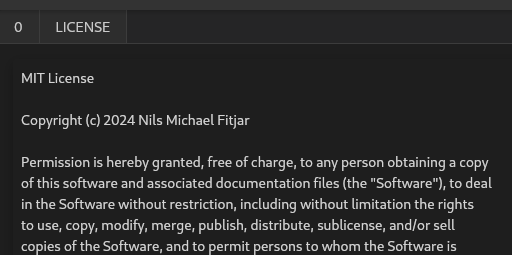
\includegraphics[width=0.75\textwidth]{./pics/tabs.png}
    \caption{
      Tab bar with two options
    }
    \end{subfigure}
    \hfill
    \begin{subfigure}[h]{0.45\textwidth}
    \centering
    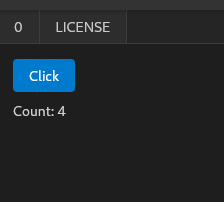
\includegraphics[width=0.5\textwidth]{./pics/tab-switch.png}
    \caption{
      After clicking on the leftmost tab, the view is changed
    }
    \end{subfigure}
  \end{figure}
\end{frame}

\begin{frame}
  \frametitle{Error reporting}
  \begin{figure}
    \centering
    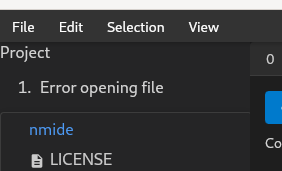
\includegraphics[width=0.5\textwidth]{./pics/errors.png}
    \caption{
      Error notification from another module
    }
  \end{figure}
\end{frame}

\begin{frame}
  \frametitle{File explorer}
  \begin{figure}
    \centering
    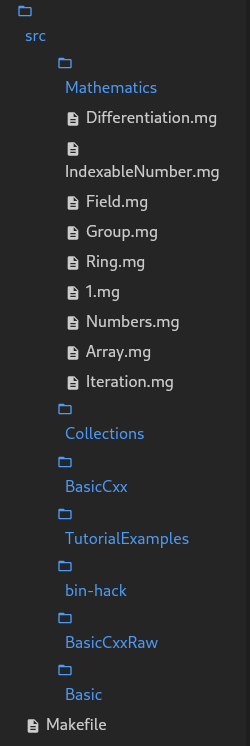
\includegraphics[height=0.5\textwidth]{./pics/ide-explorer.png}
    \caption{
      File explorer module
    }
  \end{figure}
\end{frame}

\begin{frame}
  \frametitle{File icons}
  \begin{figure}
    \centering
    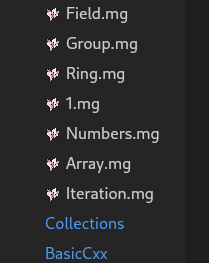
\includegraphics[width=0.35\textwidth]{./pics/file-explorer-icons.png}
    \caption{
      File explorer module, extended by a file-icon for Magnolia files
    }
  \end{figure}
\end{frame}

\begin{frame}
  \frametitle{File system operations}
  \begin{itemize}
    \item Since this IDE can target different OSes
    \item This is achieved by our module, ide\_fsa
    \item Makes file operations OS-agnostic
  \end{itemize}
\end{frame}

\begin{frame}
  \frametitle{Persistant storage}
  \begin{itemize}
    \item The core has no persistant storage
    \item A module can persist storage
    \item The core emits an exit event, giving modules a chance to block the
    core thread
    \item The same module loads the state during startup
  \end{itemize}
\end{frame}

\begin{frame}
  \frametitle{Module installer}
  \begin{figure}
    \centering
    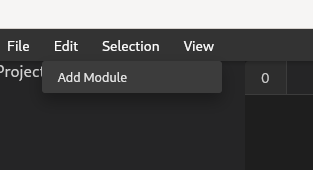
\includegraphics[width=0.5\textwidth]{./pics/module-installer-tab.png}
    \caption{
      Dropdown for adding a module
    }
  \end{figure}
  \begin{figure}
    \centering
    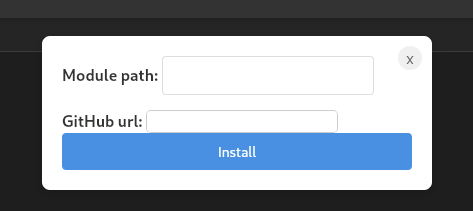
\includegraphics[width=0.5\textwidth]{./pics/module-installer.png}
    \caption{
      Form for downloading modules
    }
  \end{figure}
\end{frame}

\begin{frame}
  \frametitle{Event sender}
  \begin{figure}
    \centering
    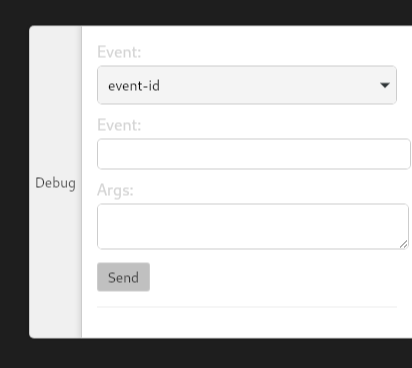
\includegraphics[width=0.5\textwidth]{./pics/event-mocking.png}
    \caption{
      Form for sending events
    }
  \end{figure}
\end{frame}

\begin{frame}
  \frametitle{State visualization}
  \begin{figure}[H]
    \begin{subfigure}[h]{0.45\textwidth}
    \centering
    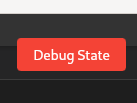
\includegraphics[height=0.25\textwidth]{./pics/debug-state-btn.png}
    \caption{
      Debug state button
    }
    \end{subfigure}
    \hfill
    \begin{subfigure}[h]{0.45\textwidth}
    \centering
    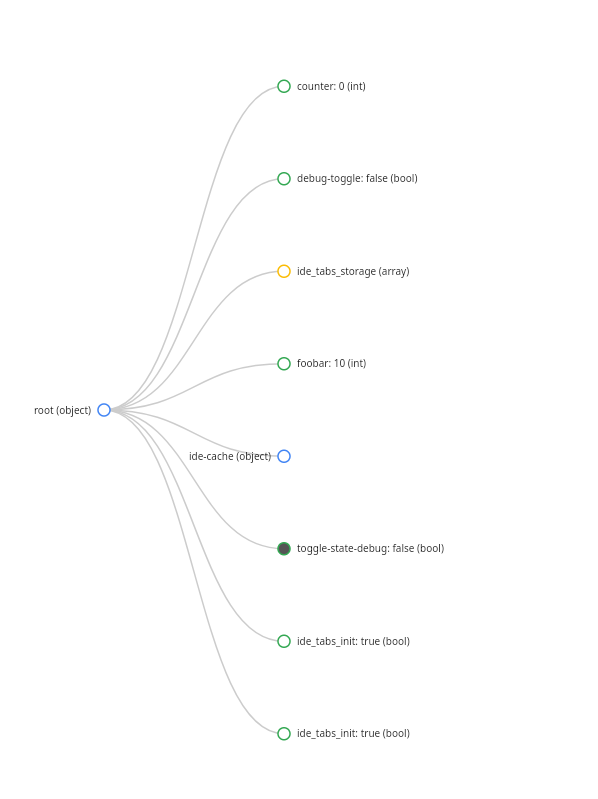
\includegraphics[height=1\textwidth]{./pics/debug-state.png}
    \caption{
      Visualization of the state
    }
    \end{subfigure}
  \end{figure}
\end{frame}

\begin{frame}
  \frametitle{Editor}
  \begin{figure}
    \centering
    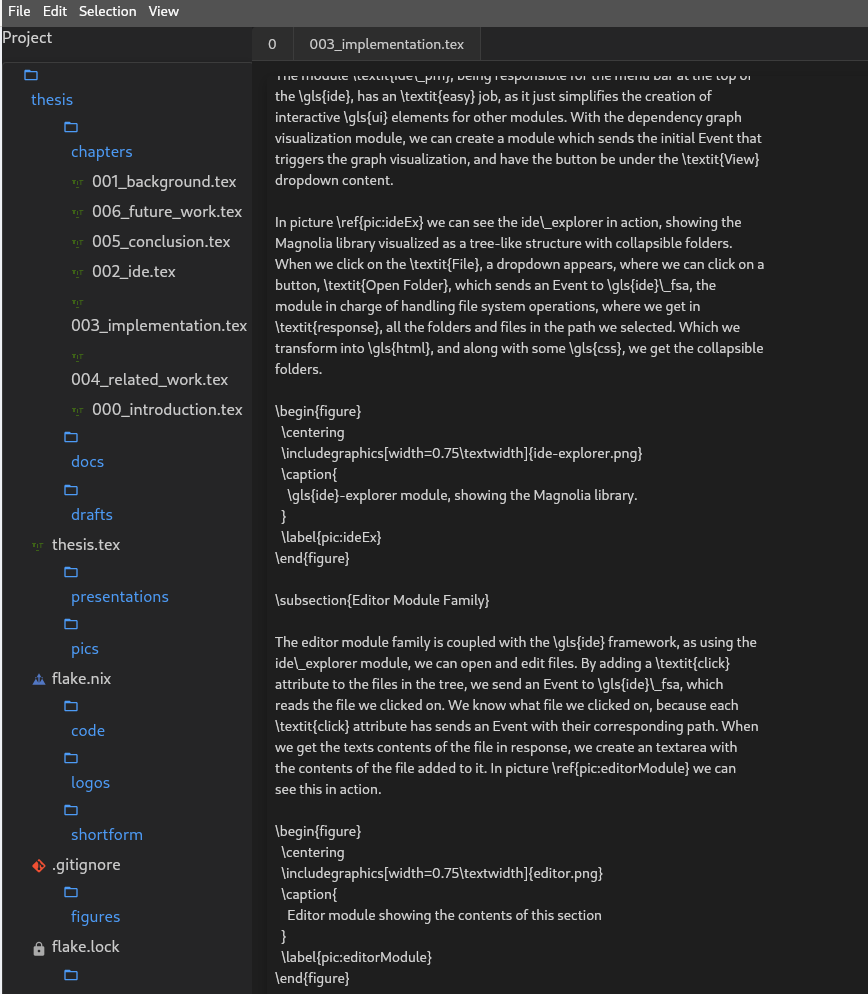
\includegraphics[width=0.5\textwidth]{./pics/editor.png}
  \end{figure}
\end{frame}

\begin{frame}
  \frametitle{Dependency vizualisation module}
  \begin{itemize}
    \item Magnolia cannot have cyclic dependencies
    \pause
    \item If any occur, the developer needs to fix it
    \pause
    \item Might be large cycles
  \end{itemize}
\end{frame}

\begin{frame}
  \frametitle{Magnolia dependency graph}
  \begin{figure}
    \centering
    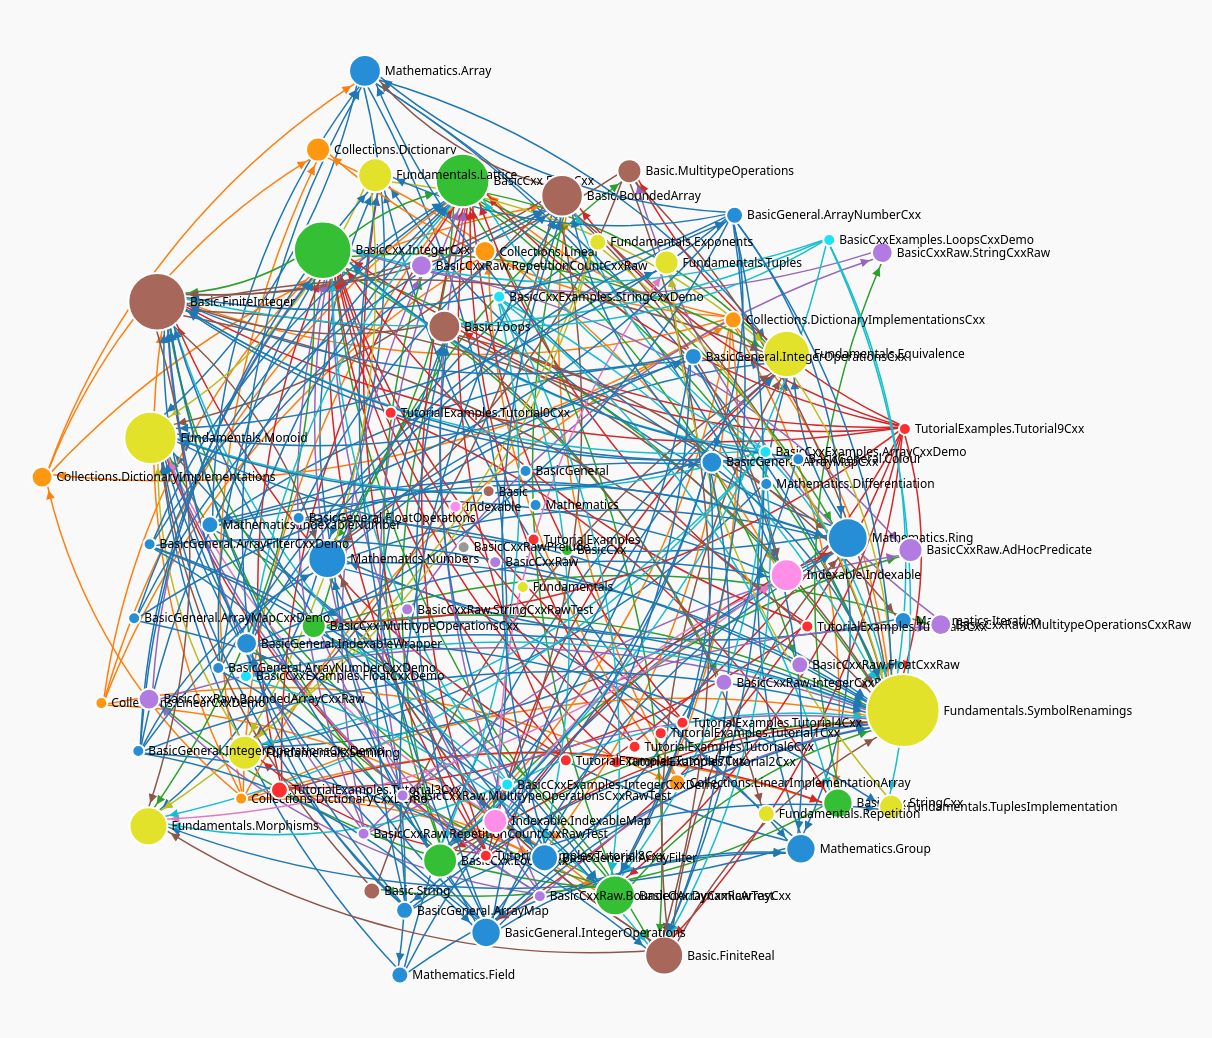
\includegraphics[width=0.75\textwidth]{./pics/magnolia-dependencies.png}
  \end{figure}
\end{frame}

\begin{frame}
  \frametitle{Rust dependencies}
  \begin{figure}
    \centering
    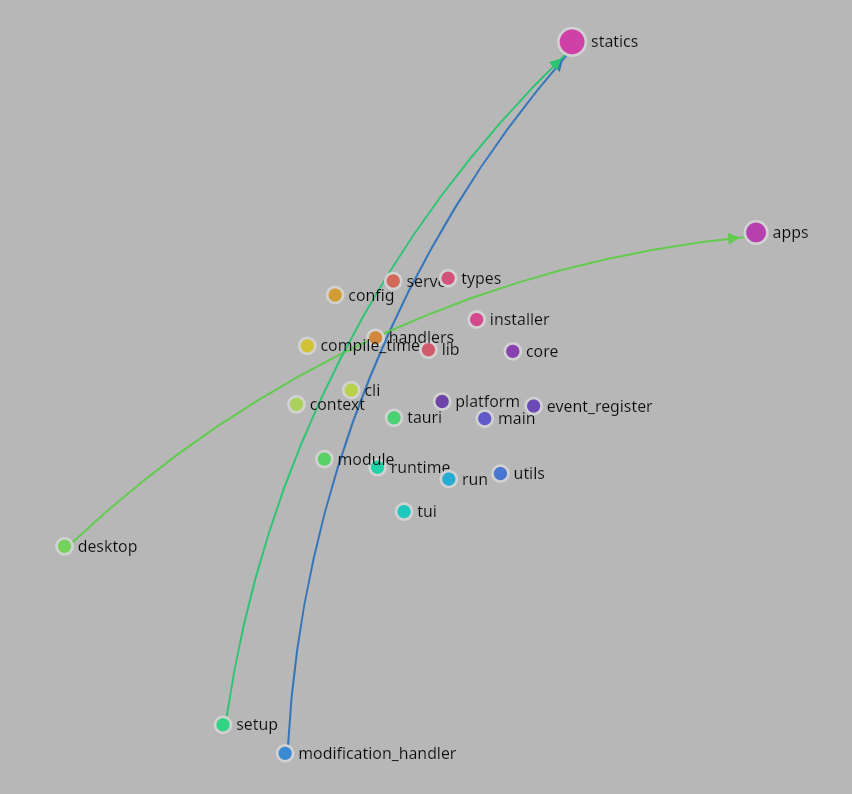
\includegraphics[width=0.5\textwidth]{./pics/rust-deps.png}
  \end{figure}
\end{frame}

\begin{frame}
  \frametitle{Module dependencies}
  \begin{figure}
    \centering
      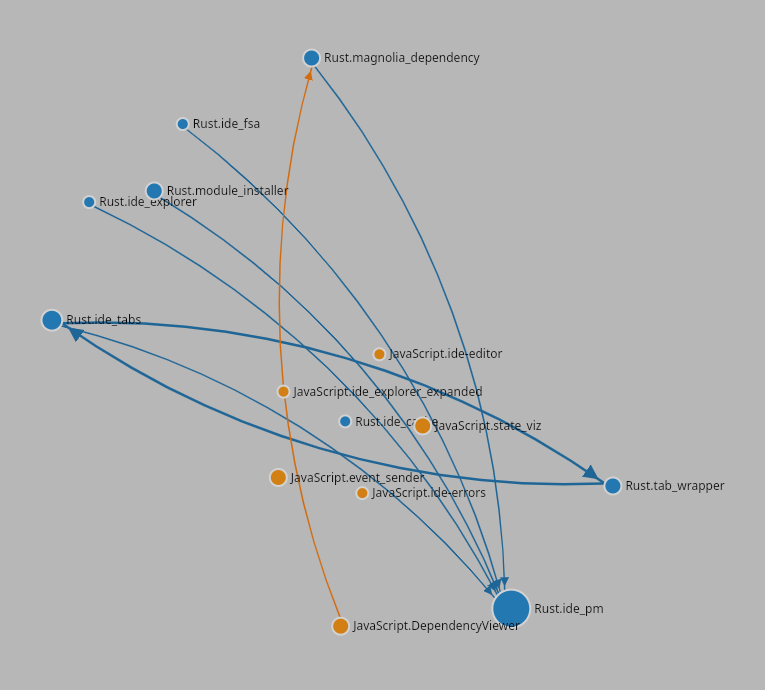
\includegraphics[width=0.7\textwidth]{./pics/module-dependencies.png}
  \end{figure}
\end{frame}
